\documentclass[../main.tex]{subfiles}
\begin{document}
\subsubsection{The many ways to derive the problem}\label{subsubsec4.1.1}
In the following we review several, equivalent methods to approach the problem of establishing the exit time of a stochastically perturbed particle sitting in a local minimum of a potential function $U(x)$ (stable equilibrium of a conservative vector field $f(x)=-\newprime{V}(x)$).
The general framework starts with a SDE in Itô form with the only assumption of the noise being additive
\begin{equation}\label{eq2.4.1.1}
     dx = f(x)dt + \sigma dW\,,
\end{equation}
and its associated FPE (or Kolmogoroff forward equation, KFE)
\begin{equation}\label{eq2.4.1.2}
     \partial_t p(x,t) = \mathcal{L}_{FP}\,p(x,t) = D\partial_{xx}^{\,2}p(x,t) - \partial_{x}\big(f(x)p(x,t)\big) = D\partial_{xx}^{\,2}p(x,t) + \partial_{x}\big(\newprime{V}(x)p(x,t)\big)\,,
\end{equation}
where $D=\frac{\sigma^{2}}{2}$ defines the diffusion coefficient.
In the following derivations we will also use the adjoint of the FP operator hence we hereby compute it. 
By definition, given a bounded, linear operator $\mathcal{L}:U\to U$ on an inner product space $U$, its adjoint $\mathcal{L}^{\dagger}$ is constructed to satisfy the relation
\begin{equation*}
     \langle \mathcal{L}p,q\rangle = \langle p,\mathcal{L}^{\dagger}q\rangle
\end{equation*}
where the bra-ket notation identifies the inner product on $V$.
A suitable choice of $V$ for the FP operator would be
\begin{equation*}
        V=\bigg\{f\in H^{1}_{0}(\mathbb{R})\;:\;\int_{-\infty}^{+\infty}fdx=1\bigg\}
\end{equation*}
i.e. it would be the space of infinetely differentiable functions which vanish at $\pm\infty$, alongside their first derivative, and whose integral is $1$ (in order to make them \textit{pdf}s).
The derivation of the adjoint follows
\begin{align*}
      \langle \mathcal{L}_{FP}p,q\rangle =& \int_{-\infty}^{+\infty}(\mathcal{L}_{FP}p(x))q(x)dx= \int_{-\infty}^{+\infty}\bigg(D \pprime{p} + \newprime{\big(\newprime{V}p\big)}\bigg)qdx = \int_{-\infty}^{+\infty}\newprime{\bigg(D \newprime{p}+\newprime{V}p\bigg)}q dx = \nonumber \\
      =& \cancelto{0}{\lim_{x\to\pm\infty}(D \newprime{p}+\newprime{V}p)q} - \int_{-\infty}^{+\infty}\bigg(D \newprime{p}+\newprime{V}p\bigg)\newprime{q} dx = -D \int_{-\infty}^{+\infty}\newprime{p}\newprime{q}dx -\int_{-\infty}^{+\infty}\newprime{V}p \newprime{q}dx =  \nonumber \\
      =& -D\bigg(\cancelto{0}{\lim_{x\to\pm\infty}p \newprime{q}}-\int_{-\infty}^{+\infty}p \pprime{q}dx\bigg)-\int_{-\infty}^{+\infty}p \newprime{V}\newprime{q}dx = \int_{-\infty}^{+\infty}p\bigg(D \pprime{q}-\newprime{V}\newprime{q}\bigg)dx = \nonumber \\
      =& \int_{-\infty}^{+\infty}p(x)(\mathcal{L}^{\dagger}_{FP}q(x))dx = \langle p,\mathcal{L}^{\dagger}_{FP}q\rangle\,.
\end{align*}
The adjoint FPE (or Kolmogoroff backward equation, KBE) thus reads
\begin{equation}\label{eq2.4.1.2.2}
     \partial_{t}p(x,t)=-\mathcal{L}^{\dagger}_{FP}p(x,t)=\newprime{V}(x)\partial_{x}p(x,t) - D\partial^{2}_{xx}p(x,t)\,.
\end{equation}
\paragraph{Derivation from first passage time}
\color{red}
(WRONG: needs review!)
\newline
Suppose you know the solution $p(x,t)$ of \eqref{eq2.4.1.2}. Suppose as well you have two subsets $\Omega_{0},\Omega_{T}\subset\Omega$ of the sample space.
The first passage time problem concerns the derivation of the probability distribution $h(t)$ of the time $t=T$ that a particle takes to reach $\Omega_{T}$ starting at time $t=0$ in $\Omega_{0}$ (henceforth referred to as \textit{hitting time distribution}).
Let us fix a specific time $t=T>0$; from the FP distribution we can compute
\begin{equation}\label{eq2.4.1.3}
     P_{T}(x\not\in \Omega_{T})=P_{T}(x\in \Omega_{T}^{\,c}) = \int_{\Omega_{T}^{\,c}}^{}p(x,t=T)dx\,,
\end{equation}
which is the probability that, at time $t=T$ the particle has not reached $\Omega_{T}$.
If instead of looking at a particular point in time we look at the entire history of the process (i.e. at any $t>0$) then Equation \eqref{eq2.4.1.3} will read
\begin{equation}\label{eq2.4.1.4}
     S(t) = \int_{\Omega_{T}^{\,c}}^{}p(x,t)dx\,,
\end{equation}
which gives us a marginal probability distribution of the time of survival of the particle (see Figure \ref{fig2.4.1.1.a}).
\begin{figure}[H]
    \centering 
    \begin{subfigure}[b]{0.325\textwidth}
        \centering 
        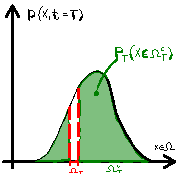
\includegraphics[keepaspectratio, width = \linewidth]{../figures/fig2.4.1.1.a.pdf}
        \caption{}
        \label{fig2.4.1.1.a}
    \end{subfigure}
    %\hfill
    \begin{subfigure}[b]{0.325\textwidth}
        \centering 
        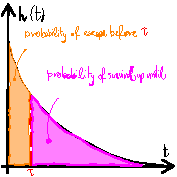
\includegraphics[keepaspectratio, width = \linewidth]{../figures/fig2.4.1.1.b.pdf}
        \caption{}
        \label{fig2.4.1.1.b}
    \end{subfigure}
    \caption{}
    \label{fig2.4.1.1}
\end{figure}
Now suppose instead that you already know the hitting time distribution $h(t)$.
Again let us fix $t=T>0$; the following quantifies the probability of the particle reaching $\Omega_{T}$ before $T$
\begin{equation}\label{eq2.4.1.5}
     P_{T}(x\in \Omega_{T}) = \int_{0}^{T}h(t)dt\,.
\end{equation}
From Equation \eqref{eq2.4.1.5} we can easily recover the probability of survival up to time $T$
\begin{align}
      P_{T}(x\in \Omega_{T}^{\,c}) =& 1 - P_{T}(x\in \Omega_{T}) = \int_{0}^{+\infty}h(t)dt - \int_{0}^{T}h(t)dt \nonumber \\
      =& \bigg(\cancel{\int_{0}^{T}h(t)dt} + \int_{T}^{+\infty}h(t)dt \bigg) - \cancel{\int_{0}^{T}h(t)dt} = \int_{T}^{+\infty}h(t)dt \,. \label{eq2.4.1.6}
\end{align}
As we did in Equation \eqref{eq2.4.1.4}, we now let $t$ to vary and therefore we recover the same distribution of survival time for our particle
\begin{equation}\label{eq2.4.1.7}
     S(t) = \int_{t}^{+\infty}h(\tau)d\tau\,.
\end{equation}
If we differentiate Equation \eqref{eq2.4.1.7} w.r.t. time we get
\begin{equation}\label{eq2.4.1.8}
        \partial_{t}S(t) = \int_{t}^{+\infty}\frac{\partial}{\partial\tau} h(\tau)d\tau = \cancelto{0}{\bigg(\lim_{\tau\to+\infty}h(\tau)\bigg)} - h(t) = -h(t)\,,
\end{equation}
and if we differentiate Equation \eqref{eq2.4.1.4} w.r.t. time we get
\begin{equation}\label{eq2.4.1.9}
        \partial_{t}S(t) = \int_{\Omega_{T}^{\,c}}^{}\partial_{t}\,p(x,t)dx \stackrel{\text{Eq.}\eqref{eq2.4.1.2}}{=}\int_{\Omega_{T}^{\,c}}^{}\mathcal{L}_{FP}\, p(x,t)dx\,.
\end{equation}
So from the equality of Equation \eqref{eq2.4.1.8} and \eqref{eq2.4.1.9} we get
\begin{equation}\label{eq2.4.1.10}
     h(t) = -\int_{\Omega_{T}^{\,c}}^{}\mathcal{L}_{FP}\, p(x,t)dx\,.
\end{equation}
Equation \eqref{eq2.4.1.10} says that the marginal w.r.t. the sample space (the complement of the target set to be precise) of the FP operator gives us the distribution of first passage time from $\Omega_{0}$ to $\Omega_{T}$.
However, to assemble $h(t)$ in practice we will need to first know $p(x,t)$, then compute its FP functional $\mathcal{L}_{FP}\, p(x,t)$ and finally compute the marginal of that. 
In most cases we will not be able to compute $p(x,t)$ explicitly.
From the definition of the $n-$th central moment of $h(t)$
\begin{equation*}
        E(t^{n})=\int_{0}^{+\infty}t^{n}h(t)dt\stackrel{\text{Eq.}\eqref{eq2.4.1.10}}{=}-\int_{0}^{+\infty}t^{n}\bigg(\int_{\Omega_{T}^{\,c}}^{}\mathcal{L}_{FP}\, p(x,t)dx\bigg)dt = -\int_{0}^{+\infty}t^{n}\partial_{t}\bigg(\int_{\Omega_{T}^{\,c}}^{}\, p(x,t)dx\bigg)dt\,,
\end{equation*}
we set $n=1$ and write the mean of $h(t)$, which we label the \textit{mean first passage time} or \textit{MFPT}
\begin{equation}\label{eq2.4.1.11}
        E(t)=\langle t\rangle =: T = -\int_{0}^{+\infty}\underbrace{t^{n}}_{u(t)}\underbrace{\partial_{t}\bigg(\int_{\Omega_{T}^{\,c}}^{}\, p(x,t)dx\bigg)}_{\newprime{v}(t)}dt\,. 
\end{equation}
We can integrate Equation \eqref{eq2.4.1.11} by parts to get
\begin{align}
        T =& \cancelto{0}{\bigg[u(t)v(t)\bigg]_{0}^{+\infty}} - \int_{0}^{+\infty}\newprime{u}(t)v(t)dt = \int_{0}^{+\infty}\bigg(\int_{\Omega_{T}^{\,c}}^{}\,p(x,t)dx\bigg)dt = \int_{\Omega_{T}^{\,c}}^{}\bigg(\underbrace{\int_{0}^{+\infty}\,p(x,t)dt}_{G(x)}\bigg)dx = \nonumber \\
          =&  \int_{\Omega_{T}^{\,c}}^{}G(x)dx\,, \label{eq2.4.1.12} 
\end{align}
where in the first step we assumed that $\lim_{t\to\infty} v(t)=\lim_{t\to\infty} \int_{\Omega_{T}^{\,c}}^{}\,p(x,t)dx = 0$, i.e. the probability of the particle to stay bounded vanishes after long enough time.
Equation \eqref{eq2.4.1.12} tells us that, in order to find the MFPT, we need to derive the marginal distribution of the states $G(x)$ across the entire history.
This is in general difficult to do since the FP distribution is unknown; instead we trade-off the explicit definition of the MFPT in order to simplify the RHS of Equation \eqref{eq2.4.1.12}.
By applying the FP operator to both sides we get
\begin{align}\label{eq2.4.1.13}
        \mathcal{L}_{FP}T(x) &= \int_{\Omega_{T}^{\,c}}^{}\mathcal{L}_{FP}G(x)dx\stackrel{\text{Eq.}\eqref{eq2.4.1.2}}{=}\int_{\Omega_{T}^{\,c}}^{}\partial_{t}G(x)dx=\int_{\Omega_{T}^{\,c}}^{}\bigg(\int_{0}^{+\infty}\partial_{t}p(x,t)dt\bigg)dx= \nonumber \\
                          &= \int_{\Omega_{T}^{\,c}}^{}\bigg(\lim_{t\to+\infty}p(x,t)-p(x,0)\bigg)dx = \cancelto{0}{\lim_{t\to+\infty}\int_{\Omega_{T}^{\,c}}^{}p(x,t)dx}-\int_{\Omega_{T}^{\,c}}^{}p(x,0)dx = \nonumber \\
                          &= -\int_{\Omega_{T}^{\,c}}^{}p(x,0)dx = -\int_{\Omega_{T}^{\,c}}^{}\delta(x)dx = -1\,,
\end{align}
where the IC $p(x,0)=\delta(x)$ is chosen to be deterministic.
Solutions of the second-order ODE \eqref{eq2.4.1.13} will give the state distribution of the MFPT conditioned on the starting state $x\in\Omega_{0}$.
Written explicitly the ODE reads
\begin{equation}\label{eq2.4.1.14}
     D \pprime{T}(x)+\newprime{(\newprime{V}(x)T(x))}=-1\,,
\end{equation}
where for the first time we introduce the potential function $V(x)$ prescribing the dynamics of the particle through its (deterministic) drift term $f(x)=-\newprime{V}(x)$.
In order to solve \eqref{eq2.4.1.14} we can consider a $1-$dimensional domain $\Omega\equiv \mathbb{R}$ while we set $\Omega_{0}=\{-\infty<x<b\}$ with $b$ being the (local) maximum of $V(x)$ (i.e. the unstable equilibrium of $f(x)$) and $\Omega_{T}=\{b\leq x<+\infty\}$.
This choice entails that the local minimum $x=a$ of the potential is found somewhere in $\Omega_{0}$ which, being bounded from above by $b$, is the basin of attraction of $a$. 
As such we can specify the following BCs for our desired mean escape time
\begin{align*}
                   T(x=b)&=0\,,\quad \text{(i.e. at the unstable equilibrium the escape occurs immediatebly),}\\
        \newprime{T}(x=b)&=0\,,\quad \text{(the mean escape time at $x=b$ is a minima of the time distribution).}\\
\end{align*}
With the above we can integrate \eqref{eq2.4.1.14} between an arbitrary $x\in\Omega_{0}$ and the unstable equilibrium $b$ bounding the basin of attraction
\begin{align}\label{eq2.4.1.15}
        \int_{x}^{b}\Big(D \pprime{T}(y)+\newprime{(\newprime{V}(y)T(y))}\Big)dy &= D(\cancelto{0}{\newprime{T}(b)}-\newprime{T}(x))+\Big(\newprime{V}(b)\cancelto{0}{T(b)}-\newprime{V}(x)T(x)\Big) = -D \newprime{T}(x)-\newprime{V}(x)T(x) = \nonumber \\
                                                                                 &= -\int_{x}^{b}1dx = -(b-x) \quad\Rightarrow\quad \newprime{T}(x)+\frac{\newprime{V}(x)}{D}T(x)=\frac{x-b}{D}\,,
\end{align}
The first-order ODE in \eqref{eq2.4.1.15} can be solved explictly using Theorem \ref{thm2.3.4.1}.
The integrating factor is readily computed
\begin{equation*}
     I(x) = e^{\int_{}^{}\frac{\newprime{V}(x)}{D}dx}=e^{\frac{V(x)}{D}}\,.
\end{equation*}
Multiplying both sides of Equation \eqref{eq2.4.1.15} by $I(x)$ and integrating gives
\begin{equation}\label{eq2.4.1.15.2}
        \int_{}^{}\newprime{(T(x)I(x))}dx = T(x)I(x) - C =\int_{}^{}\frac{x-b}{D}I(x)dx \quad\Rightarrow\quad T(x) = \frac{\int_{}^{}\frac{x-b}{D}e^{\frac{V(x)}{D}}dx+C}{e^{\frac{V(x)}{D}}}\,.
\end{equation}
To derive the constant of integration $C$ in Equation \eqref{eq2.4.1.15.2} we impose the aforementioned BC at $x=b$
\begin{equation}\label{eq2.4.1.15.3}
        T(x=b)=0=\frac{\int_{}^{}\cancelto{0}{\frac{b-b}{D}}e^{\frac{V(x)}{D}}dx+C}{e^{\frac{V(b)}{D}}} \quad\Rightarrow\quad C=0 \quad\Rightarrow\quad T(x)=e^{-\frac{V(x)}{D}}\int_{}^{}\frac{x-b}{D}e^{\frac{V(x)}{D}}dx\,,
\end{equation}
The closed form above gives the \textit{MFPT} implicitly.
To derive an explicit expression we can expand the potential in a Taylor series centered around its local maximum $x=b$ 
\begin{equation*}
     V(x) = V(b)+\cancelto{0}{\newprime{V}(b)}(x-b)+\frac{\pprime{V}(b)}{2}(x-b)^{2}+\mathcal{O}(x^{3})\,,
\end{equation*}
\begin{equation*}
        e^{\frac{V(x)}{D}} \approx e^{\frac{1}{D}\big(V(b)+\frac{\pprime{V}(b)}{2}(x-b)^{2}\big)}\,, 
\end{equation*}
which plugged into Equation \eqref{eq2.4.1.15.3} yields
\begin{align}
        T(x) &\approx e^{-\frac{V(x)}{D}}\bigg(\int_{}^{}\frac{x-b}{D}e^{\frac{1}{D}\big(V(b)+\frac{\pprime{V}(b)}{2}(x-b)^{2}\big)}dx\bigg) = e^{-\frac{V(x)}{D}}\bigg(e^{\frac{V(b)}{D}}\int_{}^{}\frac{x-b}{D}e^{\frac{\pprime{V}(b)}{2D}(x-b)^{2}}dx\bigg) = \nonumber \\
             &= e^{-\frac{V(x)}{D}}\bigg(\frac{e^{\frac{V(b)}{D}}}{\pprime{V}(b)}\int_{}^{}\frac{d}{dx}\Big(e^{\frac{\pprime{V}(b)}{2D}(x-b)^{2}}\Big)dx\bigg) = e^{-\frac{V(x)}{D}}\bigg(\frac{e^{\frac{V(b)}{D}}}{\pprime{V}(b)}\Big(e^{\frac{\pprime{V}(b)}{2D}(x-b)^{2}} + C\Big)\bigg)\nonumber \\
             &=  \frac{e^{\frac{\Delta V(x)}{D}}}{\pprime{V}(b)}\Big(e^{\frac{\pprime{V}(b)}{2D}(x-b)^{2}} + C\Big)\stackrel{T(b)=0}{=}\frac{e^{\frac{\Delta V(x)}{D}}}{\pprime{V}(b)}\Big(e^{\frac{\pprime{V}(b)}{2D}(x-b)^{2}} - 1\Big)\,,\quad\Delta V(x)=V(b)-V(x)\,. \label{eq2.4.1.15.4}
\end{align}
\color{black}
\paragraph{Derivation from the (stationary and homogeneous) probability current}
We start by rewriting the FPE \eqref{eq2.4.1.2} in terms of the probability density current $J(x,t)$
\begin{equation}\label{eq2.4.1.16}
     \partial_{t}p(x,t)=D\partial_{xx}^{2}p(x,t)+\partial_{x}(\newprime{V}(x)p(x,t))=\partial_{x}(D\partial_{x}p(x,t)+\newprime{V}(x)p(x,t))=\partial_{x}J(x,t)\,.
\end{equation}
We now proceed by rewriting the probability current itself
\begin{align*}
        J(x,t) &= D\partial_{x}p(x,t)+\newprime{V}(x)p(x,t) = D e^{-\frac{V(x)}{D}}\bigg(e^{\frac{V(x)}{D}}\partial_{x}p(x,t) + \underbrace{\frac{\newprime{V}(x)}{D}e^{\frac{V(x)}{D}}}_{\partial_{x}e^{\frac{V(x)}{D}}}p(x,t)\bigg) = \nonumber \\ 
               &= D e^{-\frac{V(x)}{D}}\bigg(e^{\frac{V(x)}{D}}\partial_{x}p(x,t) + p(x,t)\partial_{x}e^{\frac{V(x)}{D}}\bigg)=D e^{-\frac{V(x)}{D}}\partial_{x}\bigg(e^{\frac{V(x)}{D}}p(x,t)\bigg)\,, \nonumber 
\end{align*}
from which we get
\begin{equation}\label{eq2.4.1.17}
    \partial_{x}\bigg(e^{\frac{V(x)}{D}}p(x,t)\bigg) = D^{-1}J(x,t)e^{\frac{V(x)}{D}}\,.
\end{equation}
To further develop the calculations we assume that $x=a$ is a local minima of $V(x)$ (i.e. a stable equilibrium for the vector field $f(x)$) so that, integrating \eqref{eq2.4.1.17} between $a$ and an arbitrary $x>a$ yields
\begin{equation}\label{eq2.4.1.18}
     e^{\frac{V(x)}{D}}p(x,t) - e^{\frac{V(a)}{D}}p(a,t)=\frac{1}{D}\int_{a}^{x}J(y,t)e^{\frac{V(y)}{D}}dy\,.
\end{equation}
From Equation \eqref{eq2.4.1.18} we can first assume stationarity of the stochastic process ($\partial_{t}p(x,t)=0=\partial_{x}J(x,t)\;\Rightarrow\;J(x,t)=J$) which will thus evolve in a bounded region around the stable equilibrium $x=a$.
As such if we define $x=b>a$ as the unstable equilibrium, then for any $x>b$, we can reasonably assume that $e^{\frac{V(t)}{D}}\gg p(x,t)\approx0$ (see Figure \ref{fig2.4.1.2.a}), and thus we retrieve
\begin{equation}\label{eq2.4.1.19}
     -e^{\frac{V(a)}{D}}p(a)=\frac{J}{D}\int_{a}^{x}e^{\frac{V(y)}{D}}dy\quad\Rightarrow\quad J = \frac{-De^{\frac{V(a)}{D}}p(a)}{\int_{a}^{x}e^{\frac{V(y)}{D}}dy}\,,\;\;\forall x\geq b\,.
\end{equation}
\begin{figure}[H]
    \centering 
    \begin{subfigure}[b]{0.325\textwidth}
        \centering 
        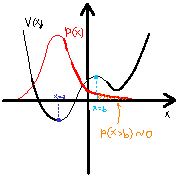
\includegraphics[keepaspectratio, width = \linewidth]{../figures/fig2.4.1.2.a.pdf}
        \caption{}
        \label{fig2.4.1.2.a}
    \end{subfigure}
    %\hfill
    \begin{subfigure}[b]{0.325\textwidth}
        \centering 
        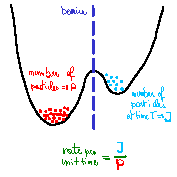
\includegraphics[keepaspectratio, width = \linewidth]{../figures/fig2.4.1.2.b.pdf}
        \caption{}
        \label{fig2.4.1.2.b}
    \end{subfigure}
    \caption{}
    \label{fig2.4.1.2}
\end{figure}
We can now switch our interpretation of the probability density current from a sample path perspective to an ensemble one (under the ergodic assumption).
From this point the probability of the stochastic process' realizations to be bounded in a region centered around the local minima $x=a$ is the total number of an ensemble of the same family of processes that at time $t$ are within such region.
If we call such probability as $P:=\int_{a-\epsilon}^{a+\epsilon}p(x,t)dx$ and interpret $J$ as the flux per unit time of trajectories in the ensemble that cross the potential barrier at $x=b$ to escape (see Figure \ref{fig2.4.1.2.b}), then we trivially derive the escape rate per unit $R$ as
\begin{equation}\label{eq2.4.1.20}
     R = \frac{J}{P}=\frac{\frac{-De^{\frac{V(a)}{D}}p(a)}{\int_{a}^{x}e^{\frac{V(y)}{D}}dy}}{\int_{a-\epsilon}^{a+\epsilon}p(x)dx}\,.
\end{equation}
Since we assumed stationarity for our process, we can rewrite the FP solution using Theorem \ref{thm2.3.4.3} as $p(x)=N e^{-\frac{V(x)}{D}}$.
Furthermore in the \textit{low-noise regime} $D\ll\Delta V(x) = V(x)-V(a)$ we can obtain an approximation of the normalisation constant and thus rewrite the stationary distribution as $p(x)=p(a)e^{-\frac{\Delta V(x)}{D}}$.
When using this assumption, the term $P$ in Equation \eqref{eq2.4.1.20} becomes
\begin{equation}\label{eq2.4.1.21}
     P=\int_{a-\epsilon}^{a+\epsilon}p(x)dx=p(a)e^{\frac{V(a)}{D}}\int_{a-\epsilon}^{a+\epsilon}e^{-\frac{V(x)}{D}}dx\,.
\end{equation}
In order to compute the integral in Equation \eqref{eq2.4.1.21} we expand the integrand in its Taylor series centered around $x=a$
\begin{equation*}
        V(x) = V(a)+\cancelto{0}{\newprime{V}(a)}(x-a)+\frac{\pprime{V}(a)}{2}(x-a)^{2}+\mathcal{O}(x^{3})\,,
\end{equation*}
\begin{equation*}
        e^{-\frac{V(x)}{D}} \approx e^{-\frac{1}{D}\big(V(a)+\frac{\pprime{V}(a)}{2}(x-a)^{2}\big)}\,, 
\end{equation*}
which gives us
\begin{align}
        P &\approx p(a)e^{\frac{V(a)}{D}}\int_{a-\epsilon}^{a+\epsilon}e^{-\frac{1}{D}\big(V(a)+\frac{\pprime{V}(a)}{2D}(x-a)^{2}\big)}dx = p(a)\cancel{e^{\frac{V(a)}{D}}}\int_{a-\epsilon}^{a+\epsilon}\cancel{e^{-\frac{V(a)}{D}}}e^{\frac{\pprime{V}(a)}{2D}(x-a)^{2}}dx = \nonumber \\
          &= p(a)\int_{a-\epsilon}^{a+\epsilon}e^{\frac{(x-a)^{2}}{\frac{2D}{\pprime{V}(a)}}}dx =p(a)\sqrt{\frac{2\pi D}{\pprime{V}(a)}} \,. \label{eq2.4.1.22}
\end{align}
Plugging Equation \eqref{eq2.4.1.22} in \eqref{eq2.4.1.20} results in
\begin{equation}\label{eq2.4.1.23}
        R = \frac{-De^{\frac{V(a)}{D}}\cancel{p(a)}}{\cancel{p(a)}\sqrt{\frac{2\pi D}{\pprime{V}(a)}}}\frac{1}{\int_{a}^{x}e^{\frac{V(y)}{D}}dy} = \frac{-De^{\frac{V(a)}{D}}\sqrt{\frac{\pprime{V}(a)}{2\pi D}}}{\int_{a}^{x}e^{\frac{V(y)}{D}}dy} \,,
\end{equation}
and finally the integral at the denominator of Equation \eqref{eq2.4.1.23} can be approximated by repeating the same Taylor expansion of $V(x)$ carried out above only this time centered around $a<b<x$
\begin{equation}\label{eq2.4.1.24}
        R \approx \frac{-De^{\frac{V(a)}{D}}\sqrt{\frac{\pprime{V}(a)}{2\pi D}}}{e^{\frac{V(b)}{D}}\sqrt{\frac{2\pi D}{\pprime{V}(b)}}} = \frac{D}{2\pi}\sqrt{\pprime{V}(a)\pprime{V}(b)}\,e^{-\frac{\Delta V}{D}}\,.
\end{equation}
where we defined $\Delta V=V(b)-V(a)$ to be the height of the (potential) barrier.
\paragraph{Derivation from the conditional solution of the FPE}
This method is similar to the first one we derived at the beginning of this paragraph in the sense that it also treats the problem from the perspective of \textit{first passage time}.
The main difference in what follows is the use of the conditional FPE and the imposition of absorbing BCs.
As such we reformulate Equation \eqref{eq2.4.1.2} as an IBVP
\begin{equation}\label{eq2.4.1.25}
   \begin{cases}
      \partial_{t}p(x,t|x_{0}, t_{0})=\mathcal{L}_{FP}p(x,t|x_{0},t_{0}) \,,\quad x\in\Omega \\
      p(x,t_{0}|x_{0},t_{0})=\delta(x-x_{0}) \,,\quad x\in\Omega\quad\text{(deterministic) IC}\,, \\
      p(x,t|x_{0}, t_{0})=0\,,\quad x\in\partial\Omega\quad\text{(absorbing) BC}\,,
   \end{cases}
\end{equation}
where, due to the absorbing BC we can deduce that
\begin{equation*}
        \lim_{t\to+\infty}p(x,t|x_{0},t_{0})=0\,,
\end{equation*}
i.e. in the time asymptotic limit any trajectory starting inside $\Omega$ would eventually hit its boundary $\partial\Omega$ and get absorbed (escape).
For a finite time $t<\infty$ however, we can compute the probability of a stochastic process to stay bounded in $\Omega$ by summing over all possible states $x\in\Omega$
\begin{equation}\label{eq2.4.1.26}
     S(t|x_{0},t_{0})=\int_{\Omega}^{}p(x,t|x_{0},t_{0})dx\,.
\end{equation}
Notice that Equation \eqref{eq2.4.1.26} quantifies the same survival time distribution that we defined in Equation \eqref{eq2.4.1.4} with the only difference of being conditioned on the starting point of the process being $x_{0}\in\Omega$ at time $t=t_{0}$.
Similarly to what we did in the first derivation, we can define such probability also in terms of the marginal of the distribution $h(t|x_{0},t_{0})$ of the \textit{hitting times}
\begin{equation}\label{eq2.4.1.27}
     S(t|x_{0},t_{0})=\int_{t}^{+\infty}h(\tau|x_{0},t_{0})d\tau\,,
\end{equation}
which corresponds to Equation \eqref{eq2.4.1.7}.
The FTC for Equation \eqref{eq2.4.1.27} then gives
\begin{equation}\label{eq2.4.1.28}
     h(t|x_{0}, t_{0})=-\frac{d}{dt}S(t|x_{0}, t_{0})\,,
\end{equation}
from which, adopting the notation $x_{0}=:x$ and $t_{0}=0$ for convenience, we compute the \textit{MFPT} as done in Equation \eqref{eq2.4.1.11}
\begin{equation}\label{eq2.4.1.29}
        T(x)=-\int_{0}^{+\infty}t\frac{d}{dt}S(t|x,0)dt=\int_{0}^{+\infty}S(t|x,0)dt\stackrel{\text{Eq.}\eqref{eq2.4.1.26}}{=}\int_{0}^{+\infty}\bigg(\int_{\Omega}^{}p(y,t|x,0)dy\bigg)dt\,,
\end{equation}
where in the integration by parts we implicitly used the property of the \textit{pdf} vanishing in the time asymptotic limit due to the absorbing BCs we imposed in Equation \eqref{eq2.4.1.25}.
From here we depart from the first derivation where, in Equation \eqref{eq2.4.1.12}, we switched the order of integration and defined a marginal distribution $G(x)$ over the states across the history of the process.
Instead we observe that, if the process is Markovian, then if we assume that there are infinitely many states $x\in\Omega$ that the process can visit, in finite time $t$, from the initial state $x(t_{0})=x_{0}$ to the final state $x(t_{n})=x_{n}$, we can write the probability of being at $x_{n}$ conditioned that we start at $x_{0}$ via the Chapman-Kolmogorov equation (see Figure \ref{fig2.4.1.3}) 
\begin{equation}\label{eq2.4.1.30}
    p(x_{n},t_{n}|x_{0},t_{0})=\int_{}^{}p(x_{n}, t_{n}|x,t)p(x,t|x_{0},t_{0})dx\,,\quad t_{0}<t<t_{n}\,.
\end{equation}
Differentianting Equation \eqref{eq2.4.1.30} w.r.t. time yields
\begin{align*}
        \partial_{t}p(x_{n},t_{n}|x_{0},t_{0}) = 0 =& \int_{}^{}\partial_{t}\bigg(p(x_{n}, t_{n}|x,t)p(x,t|x_{0},t_{0})\bigg)dx = \nonumber \\
        =& \int_{}^{}\bigg(p(x,t|x_{0},t_{0})\partial_{t}p(x_{n}, t_{n}|x,t) + p(x_{n}, t_{n}|x,t)\partial_{t}p(x,t|x_{0},t_{0})\bigg)dx \stackrel{\text{Eq.}\eqref{eq2.4.1.25}}= \nonumber \\
        =& \int_{}^{}\bigg(p(x,t|x_{0},t_{0})\partial_{t}p(x_{n}, t_{n}|x,t) + p(x_{n}, t_{n}|x,t)\mathcal{L}_{FP}p(x,t|x_{0},t_{0})\bigg)dx \stackrel{\text{Eq.}\eqref{eq2.4.1.2.2}}{=} \nonumber \\
        =& \int_{}^{}\bigg(p(x,t|x_{0},t_{0})\partial_{t}p(x_{n}, t_{n}|x,t) + p(x,t|x_{0},t_{0})\mathcal{L}^{\dagger}_{FP}p(x_{n}, t_{n}|x,t)\bigg)dx = \nonumber \\
        =& \int_{}^{}\bigg(\partial_{t}p(x_{n}, t_{n}|x,t) + \mathcal{L}^{\dagger}_{FP}p(x_{n}, t_{n}|x,t)\bigg)p(x,t|x_{0},t_{0})dx\,,
\end{align*}
from which we recover the adjoint FPE in Equation \eqref{eq2.4.1.2.2}
\begin{equation*}
     \partial_{t}p(x_{n}, t_{n}|x,t) + \mathcal{L}^{\dagger}_{FP}p(x_{n}, t_{n}|x,t)=0\,.
\end{equation*}
Applying the adjoint FP operator to Equation \eqref{eq2.4.1.29} gives us an ODE for the \textit{MFPT}
\begin{align}
     \mathcal{L}^{\dagger}_{FP}T(x) =& -\int_{0}^{+\infty}\bigg(\int_{\Omega}^{}\partial_{t}p(y,t|x,0)dx\bigg)dt = -\int_{\Omega}^{}\bigg(\int_{0}^{+\infty}\partial_{t}p(y,t|x,0)dt\bigg)dx = \nonumber \\
     =& \int_{\Omega}^{}p(y,0|x,0)dx \stackrel{\text{Eq.}\eqref{eq2.4.1.25}}{=}\int_{\Omega}^{}\delta(y-x)dx = 1  \,, \label{eq2.4.1.31}
\end{align}
\begin{figure}[H]
    \centering 
    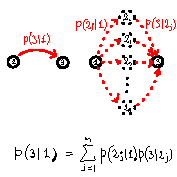
\includegraphics[keepaspectratio, width=0.5\textwidth]{../figures/fig2.4.1.3.pdf}
    \caption{}
    \label{fig2.4.1.3}
\end{figure}
Written explicitly the ODE in Equation \eqref{eq2.4.1.31} reads
\begin{equation}\label{eq2.4.1.32}
     D \pprime{T}(x)-\newprime{V}(x)\newprime{T}(x)=1\,,
\end{equation}
which we notice it is the adjoint of Equation \eqref{eq2.4.1.14}.
Similarly to what we did in the derivation from the stationary probability current, we multiply both sides of \eqref{eq2.4.1.32} by $\frac{e^{-\frac{V(x)}{D}}}{D}$ and proceed by algebraic manipulation to get
\begin{align}
     \frac{e^{-\frac{V(x)}{D}}}{D} =& e^{-\frac{V(x)}{D}}\frac{d^{2}}{dx^{2}}T(x) - \frac{\newprime{V}}{D}(x)e^{-\frac{V(x)}{D}}\frac{d}{dx}T(x) = e^{-\frac{V(x)}{D}}\frac{d^{2}}{dx^{2}}T(x) + \bigg(\frac{d}{dx}e^{-\frac{V(x)}{D}}\bigg)\bigg(\frac{d}{dx}T(x)\bigg) = \nonumber \\
                                   =& \frac{d}{dx}\bigg(e^{-\frac{V(x)}{D}}\frac{d}{dx}T(x)\bigg)\,, \label{eq2.4.1.33}
\end{align}
We now assume that the potential landscape has a form as depicted in Figure \ref{fig2.4.1.2.a}, i.e. it has a local minimum in $x=a>-\infty$ and a local maximum at $+\infty>x=b>a$.
As such, integrating \eqref{eq2.4.1.33} in $[-\infty,x]$ yields
\begin{equation*}
         e^{-\frac{V(x)}{D}}\frac{d}{dx}T(x) - \cancelto{0}{\lim_{x\to-\infty}e^{-\frac{V(x)}{D}}\frac{d}{dx}T(x)}= \frac{1}{D}\int_{-\infty}^{x}e^{-\frac{V(y)}{D}}dy\,,
\end{equation*}
and integrating again in $[x,b]$ gives us an implicit expression for the \textit{MFPT}
\begin{equation}\label{eq2.4.1.34}
        \cancelto{0}{T(b)} - T(x) =\frac{1}{D}\int_{x}^{b}e^{\frac{V(y)}{D}}\bigg(\int_{-\infty}^{y}e^{-\frac{V(z)}{D}}dz\bigg)dy\,.
\end{equation}
By recalling the Taylor expansion of the potential function around a stationary point $x=c\in\{a,b\}$ we have
\begin{align*}
     e^{\frac{V(y)}{D}} \approx& \; e^{\frac{1}{D}\big(V(b)+\frac{\pprime{V}(b)}{2}(x-b)^{2}\big)} \nonumber \\
      e^{-\frac{V(z)}{D}} \approx& \; e^{-\frac{1}{D}\big(V(a)+\frac{\pprime{V}(a)}{2}(x-a)^{2}\big)} \,, \nonumber
\end{align*}
which, plugged in Equation \eqref{eq2.4.1.34}, yields the closed form for the \textit{MFPT}
\begin{align}
        -T(x) \approx& \frac{1}{D}\int_{x}^{b}e^{\frac{V(b)}{D}}e^{\frac{\pprime{V}(b)}{2}(y-b)^{2}}\bigg(\int_{-\infty}^{y}e^{-\frac{V(a)}{D}}e^{-\frac{\pprime{V}(a)}{2}(z-a)^{2}}dz\bigg)dy = \nonumber \\
                   =& \frac{e^{\frac{V(b)-V(a)}{D}}}{D}\int_{x}^{b}e^{\frac{\pprime{V}(b)}{2}(y-b)^{2}}\bigg(\int_{-\infty}^{y}e^{-\frac{\pprime{V}(a)}{2}(z-a)^{2}}dz\bigg)dy \nonumber \\
                   =& \frac{e^{\frac{\Delta V}{D}}}{D}\int_{x}^{b}e^{\frac{\pprime{V}(b)}{2}(y-b)^{2}}\bigg(\int_{-\infty}^{y}e^{-\frac{\pprime{V}(a)}{2}(z-a)^{2}}dz\bigg)dy\,. \label{eq2.4.1.35}
\end{align}
We can drop the dependence on the state $x$ from Equation \eqref{eq2.4.1.35}, which implicitly assumes that the escape time is compute for a stochastic process bounded in a small neighbour of the local minimum $x=a$ of the potential function (i.e. the stable equilibrium of the vector field $f(x)=-\newprime{V}(x)$).
In doing so we can substitute the bounds of integration in the outer integral $x\mapsto-\infty$, $b\mapsto+\infty$ and the upper bound in the inner integral $y\mapsto+\infty$ thus getting
\begin{align}
     -T =&  = \frac{e^{\frac{\Delta V}{D}}}{D}\int_{-\infty}^{+\infty}e^{\frac{\pprime{V}(b)}{2}(y-b)^{2}}\bigg(\int_{-\infty}^{+\infty}e^{-\frac{\pprime{V}(a)}{2}(z-a)^{2}}dz\bigg)dy = \nonumber \\
        =& \frac{e^{\frac{\Delta V}{D}}}{D}\bigg(\int_{-\infty}^{+\infty}e^{-\big(-\frac{\pprime{V}(b)}{2}\big)(y-b)^{2}}dy\bigg)\bigg(\int_{-\infty}^{+\infty}e^{-\frac{\pprime{V}(a)}{2}(z-a)^{2}}dz\bigg) = \nonumber \\
        =& \frac{e^{\frac{\Delta V}{D}}}{D}\sqrt{\frac{2\pi}{-\pprime{V}(b)}}\sqrt{\frac{2\pi}{\pprime{V}(a)}} = \frac{2\pi}{D}\bigg(\sqrt{\pprime{V}(a)|\pprime{V}(b)|}\bigg)^{-1}e^{\frac{\Delta V}{D}} \,, \label{eq2.4.1.36}
\end{align}
where we can substitute $-\pprime{V}(b)\mapsto|\pprime{V}(b)|$ given that $\pprime{V}(b)<0$ ($x=b$ is a local maximum for $V(x)$).
By taking the inverse of \eqref{eq2.4.1.36} we recover Kramers' escape rate given by Equation \eqref{eq2.4.1.24}
\begin{equation*}
        R = -\frac{D}{2\pi}\sqrt{\pprime{V}(a)|\pprime{V}(b)|}e^{-\frac{\Delta V}{D}}\,.
\end{equation*}
\end{document}
